\documentclass{standalone}

\usepackage{tikz}
\usepackage{pgfplots}
\usetikzlibrary{calc}

\begin{document}
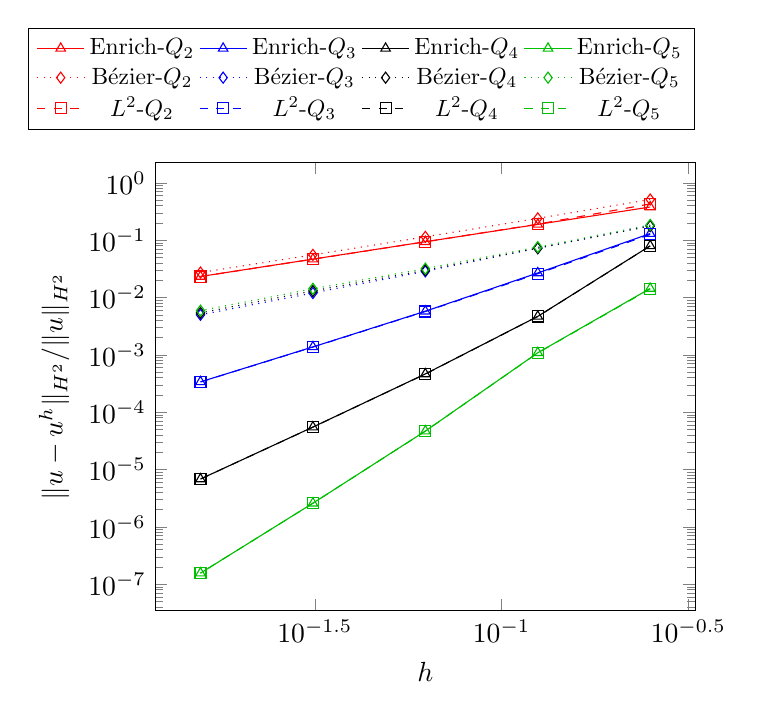
\begin{tikzpicture}
    \begin{loglogaxis}[
        legend columns=4,
    	legend style={at={(1,1.3)}, nodes={scale=.85, transform shape}},
        xlabel=$h$,
        ylabel=${\|u-u^{h}\|_{H^2}}/{\|u\|_{H^2}}$ 
    ]

    \addplot [color=red,mark=triangle] plot coordinates {

        (.25,       0.37916)
        (.125,      0.188337)
        (.0625,     0.0939535)
        (0.03125,   0.0467433)
        (0.015625,  0.0232856)
    };

    
    \addplot [color=blue,mark=triangle] plot coordinates {

        (.25,       0.130408)
        (.125,      0.0268261)
        (.0625,     0.00577062)
        (0.03125,   0.00137533)
        (0.015625,  0.000338073)
    };

    \addplot [color=black,mark=triangle] plot coordinates {

        (.25,       0.0797354)
        (.125,      0.00468696)
        (.0625,     0.000464571)
        (0.03125,   5.50219e-05)
        (0.015625,  6.82918e-06)
    };

    \addplot [color=green!75!black,mark=triangle] plot coordinates {

        (.25,       0.0144054)
        (.125,      0.00108814)
        (.0625,     4.684e-05)
        (0.03125,   2.58651e-06)
        (0.015625,  1.56118e-07)
    };

    
    \addplot [color=red,mark=diamond, every mark/.append style={solid}, dotted] plot coordinates {

        (.25,       0.511757)
        (.125,      0.240184)
        (.0625,     0.114346)
        (0.03125,   0.0554896)
        (0.015625,  0.0272939)
    };

    
    \addplot [color=blue,mark=diamond, every mark/.append style={solid}, dotted] plot coordinates {

        (.25,       0.179079)
        (.125,      0.0729287)
        (.0625,     0.0286441)
        (0.03125,   0.0119787)
        (0.015625,  0.0050)
    };

    \addplot [color=black,mark=diamond, every mark/.append style={solid}, dotted] plot coordinates {

        (.25,       0.176097)
        (.125,      0.0724466)
        (.0625,     0.0299489)
        (0.03125,   0.0130237)
        (0.015625,  0.0054)
    };

    \addplot [color=green!75!black,mark=diamond, every mark/.append style={solid}, dotted] plot coordinates {

        (.25,       0.184512)
        (.125,      0.0758842)
        (.0625,     0.031917)
        (0.03125,   0.0142136)
        (0.015625,  0.0059)
    };


    \addplot [color=red,mark=square, every mark/.append style={solid}, dashed] plot coordinates {

        (.25,       0.429158)
        (.125,      0.190387)
        (.0625,     0.0937169)
        (0.03125,   0.0465883)
        (0.015625,  0.0232335)
    };

    
    \addplot [color=blue,mark=square, every mark/.append style={solid}, dashed] plot coordinates {

        (.25,       0.125872)
        (.125,      0.0260387)
        (.0625,     0.00570847)
        (0.03125,   0.00136665)
        (0.015625,  0.000337016)
    };

    \addplot [color=black,mark=square, every mark/.append style={solid}, dashed] plot coordinates {

        (.25,       0.0794173)
        (.125,      0.00467507)
        (.0625,     0.000462874)
        (0.03125,   5.49137e-05)
        (0.015625,  6.82295e-06)
    };

    \addplot [color=green!75!black,mark=square, every mark/.append style={solid}, dashed] plot coordinates {

        (.25,       0.0141393)
        (.125,      0.00108092)
        (.0625,     4.67021e-05)
        (0.03125,   2.58318e-06)
        (0.015625,  1.56058e-07)
    };

    \logLogSlopeTriangle{0.16}{0.075}{0.06}{4}{green!75!black};
    \logLogSlopeTriangle{0.16}{0.075}{0.27}{3}{black};
    \logLogSlopeTriangle{0.16}{0.075}{0.48}{2}{blue};
    \logLogSlopeTriangle{0.16}{0.075}{0.725}{1}{red};

    \legend{Enrich-$Q_2$\\Enrich-$Q_3$\\Enrich-$Q_4$\\Enrich-$Q_5$\\B\'ezier-$Q_2$\\B\'ezier-$Q_3$\\B\'ezier-$Q_4$\\B\'ezier-$Q_5$\\$L^2$-$Q_2$\\$L^2$-$Q_3$\\$L^2$-$Q_4$\\$L^2$-$Q_5$\\}
    \end{loglogaxis}
\end{tikzpicture}

\end{document}
